\section{Results and Discussion}\label{sec:results}

\subsection{Experimental Setup}
The analysis ran in Python with NumPy~2.3.5, SciPy~1.17.0, pandas~2.3.3 and statsmodels~0.14.5 from a pinned lock file. Thirty unit tests pass, and a Docker build and a fresh-clone run reproduced the committed estimates. The benchmark log holds \vnLog{} records (\vnWarm{} warm-up, \vnBench{} timed) collected on an \vcpu{} with \vncpu{} logical CPUs and Python~\vpyBench.

\subsection{RQ1: Association}
In the main sample, GenAI-use frequency and the UPS total~\eqref{eq:ups} were positively associated: $\hat\rho_s=\vrhoMain$ by~\eqref{eq:rho}, 95\% CI \vrhoMainLo--\vrhoMainHi{} by~\eqref{eq:ci}, asymptotic $p=\vpAsymMain$. No permutation in~\eqref{eq:perm} reached the observed value, so $p_{\text{perm}}=1/(B+1)\approx10^{-4}$, and all $10^4$ bootstrap resamples were valid. $H_0$ is therefore rejected. Fig.~\ref{fig:effects} shows that the estimate barely moved in Sensitivity~A ($\hat\rho_s=\vrhoA$) and Sensitivity~B ($\hat\rho_s=\vrhoB$), the two alternative selections of Section~\ref{sec:data}, so the result does not appear to depend on the data authors' undocumented exclusions.

\begin{figure}[!t]
\centering
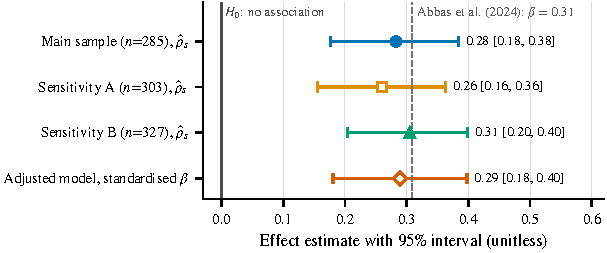
\includegraphics[width=\columnwidth]{generated/fig_effects.pdf}
\caption{Effect estimates with 95\% intervals: Spearman $\hat\rho_s$ in the three samples (bootstrap) and the standardised $\beta$ of model $M_1$ (HC3). The solid line is the null baseline; the dashed line is the estimate of Abbas et al.~\cite{abbas2024harmful}.}
\label{fig:effects}
\end{figure}

\subsection{RQ2: Comparison with Baselines}
Table~\ref{tab:baselines} compares the estimate with the statistical baselines of Section~\ref{sec:estimators}. The four frequency groups differed overall (Kruskal--Wallis $H=\vkwH$, $p<0.001$, $\varepsilon^2=\vepsSq$). Relative to the monthly reference group (median \pMedOne), students using GenAI a few times a week or every day scored 3.5--4 points higher with medium dominance ($\delta=\pDeltaThree$ and \pDeltaFour), while weekly users did not differ after Holm correction. Against the rarely-or-never group of Sensitivity~B, the corresponding $\delta$ rose to \pDeltaBThree{} and \pDeltaBFour. Adding frequency to the demographic model~\eqref{eq:models} raised $R^2$ from \vrTwoBase{} to \vrTwoProp{} ($F=\vFnested$, $p\vpNested$); each step up the frequency scale corresponded to $\beta=\vbeta$ UPS points (95\% CI \vbetaLo--\vbetaHi). The residuals were not normal (Shapiro--Wilk $p=\vshapiroP$), which supports the rank-based primary metric and the HC3 errors, and showed no clear heteroscedasticity (Breusch--Pagan $p=\vbpP$).

\begin{table}[!t]
\caption{Survey Estimates Against the Statistical Baselines}
\label{tab:baselines}
\centering
\footnotesize
\setlength{\tabcolsep}{3pt}
\begin{tabular}{@{}llll@{}}
\toprule
Baseline & Proposed & Estimate [95\% CI] & $p$ \\
\midrule
$\rho_s=0$ & Main, $\hat\rho_s$ & \vrhoMain{} [\vrhoMainLo, \vrhoMainHi] & $\vpAsymMain$ \\
$\rho_s=0$ & Sens.\ A, $\hat\rho_s$ & \vrhoA{} [\vrhoALo, \vrhoAHi] & $<0.001$ \\
$\rho_s=0$ & Sens.\ B, $\hat\rho_s$ & \vrhoB{} [\vrhoBLo, \vrhoBHi] & $<0.001$ \\
Monthly & Weekly, $\delta$ & $\pDeltaTwo$ $\pDeltaTwoCi$ & $\pHolmTwo^{\dagger}$ \\
(median \pMedOne) & Few/week, $\delta$ & $\pDeltaThree$ $\pDeltaThreeCi$ & $\pHolmThree^{\dagger}$ \\
 & Daily, $\delta$ & $\pDeltaFour$ $\pDeltaFourCi$ & $\pHolmFour^{\dagger}$ \\
$M_0$, $R^2=\vrTwoBase$ & $M_1$, $\Delta R^2$ & \vdRTwo{} ($R^2=\vrTwoProp$) & $<0.001$ \\
Abbas et al., $\beta=0.31$ & Std.\ $\beta$ & \vbetaStd{} [\vbetaStdLo, \vbetaStdHi] & --- \\
\bottomrule
\multicolumn{4}{@{}l@{}}{\scriptsize $^{\dagger}$Holm-adjusted Mann--Whitney $p$; $\delta$ is Cliff's dominance.}\\
\end{tabular}
\end{table}

\subsection{RQ3: Pipeline Performance}
Table~\ref{tab:bench} and Fig.~\ref{fig:latency} compare the two implementations under the design of Section~\ref{sec:pipeline}. The vectorised bootstrap was faster at every workload, with $\mathcal{S}$ in~\eqref{eq:speedup} falling from \vspeedMax{} at 50 records to \vspeedMin{} at 2{,}000. The loop pays a fixed cost of one library call per resample, which dominates small inputs; as $n$ grows, ranking itself dominates both versions and the gap narrows. Over \vnPaired{} paired runs on identical inputs, the largest difference between the estimates was $2.2\times10^{-16}$, no run failed unexpectedly ($e=0$), and all \vnInjected{} injected invalid batches were rejected ($d=1$).

\begin{table}[!t]
\caption{Median (p95) Latency per Analysis Call in ms}
\label{tab:bench}
\centering
\footnotesize
\begin{tabular}{@{}rccc@{}}
\toprule
Records & Loop (baseline) & Vectorised & Speed-up $\mathcal{S}$ [95\% CI] \\
\midrule
50 & \pLatLoopFifty{} (\pLatHighLoopFifty) & \textbf{\pLatVecFifty} (\pLatHighVecFifty) & \pSpeedFifty{} \pSpeedFiftyCi \\
285 & \pLatLoopTwoEightyFive{} (\pLatHighLoopTwoEightyFive) & \textbf{\pLatVecTwoEightyFive} (\pLatHighVecTwoEightyFive) & \pSpeedTwoEightyFive{} \pSpeedTwoEightyFiveCi \\
2{,}000 & \pLatLoopTwoThousand{} (\pLatHighLoopTwoThousand) & \textbf{\pLatVecTwoThousand} (\pLatHighVecTwoThousand) & \pSpeedTwoThousand{} \pSpeedTwoThousandCi \\
\bottomrule
\end{tabular}
\end{table}

\begin{figure}[!t]
\centering
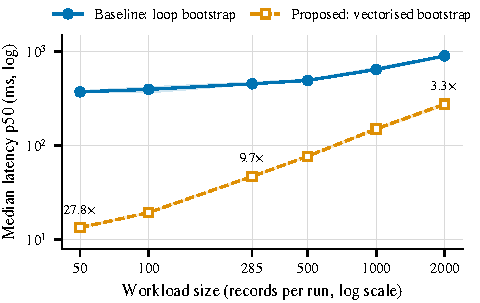
\includegraphics[width=\columnwidth]{generated/fig_latency.pdf}
\caption{Median latency against workload size (log--log). Shaded bands are 95\% bootstrap intervals of the median; labels give the speed-up $\mathcal{S}$.}
\label{fig:latency}
\end{figure}

\subsection{Discussion}\label{sec:discussion}
The results suggest a positive but modest association. By norms for individual-differences research, $\hat\rho_s\approx0.28$ sits near the ``relatively large'' range~\cite{gignac2016effect}, yet frequency explained only about 8\% of the variance in UPS totals. The estimate agrees with the cross-sectional $\beta=0.309$ of Abbas et al.~\cite{abbas2024harmful}, which lies inside our interval (Fig.~\ref{fig:effects}). The panel evidence~\cite{zhao2026panel}, however, implies that a correlation of this size may reflect stable individual differences, such as workload or self-regulation, rather than an effect of GenAI on procrastination. The plateau between use a few times a week and daily use points in the same direction: more frequent use was not associated with ever higher scores.

For Kazakhstan, the estimate is best treated as a hypothesis. With most students already using AI weekly~\cite{askarkyzy2024perceptions}, exposure would be concentrated in the upper levels, a range restriction that would tend to attenuate $\rho_s$. Within our experimental envelope, the engineering result is clearer: removing per-resample library calls gives a three- to 28-fold latency gain without changing a single reported estimate.

These findings have a practical reading. Usage frequency alone appears to be a weak marker of procrastination risk, so policies that simply restrict how often students may use GenAI are unlikely to address the behaviour. Guidance on the purpose of use and support for self-regulation, which the panel evidence links to later academic functioning~\cite{zhao2026panel}, seem more promising targets. For researchers, the pipeline shows that a full bootstrap analysis of a few hundred respondents can run in under a second, which makes repeated sensitivity analyses cheap enough to report routinely.
